\documentclass[compsoc, conference, a4paper, 10pt, times]{IEEEtran}

\usepackage{cite}
\usepackage{amsmath,amssymb,amsfonts}
\usepackage{algorithm,algorithmic}  %% typset algorithms

\usepackage{graphicx}
\usepackage{textcomp}
\usepackage{xcolor}
\usepackage{booktabs}
\usepackage[hidelinks]{hyperref}

\usepackage{amsthm}
%%\usepackage{newpxtext}  %% for _e.g._ macro.
\usepackage{textgreek}
\usepackage{xspace}
\usepackage{centernot}

% use these if you also want π to work in math mode
\usepackage{newunicodechar}
\newunicodechar{Π}{\ifmmode\Pi\else\textPi\fi}
\newunicodechar{⫫}{\mathrel{\perp\!\!\!\perp}}

% use quotes as smart-quotes. https://tex.stackexchange.com/a/52354
%\usepackage [english]{babel}
\usepackage [autostyle, english = american]{csquotes}
\MakeOuterQuote{"}
\usepackage{graphicx}

\renewcommand{\paragraph}[1]{\vspace*{2pt}\noindent\textbf{#1}}

\newcommand{\langname}{\textsc{\textbf{.}CHO}\xspace}
\newcommand{\toolname}{\textsc{DT-SIM}\xspace}

\title{Title Goes Here}

\author{First1 Last1}
%%\authornote{with author1 note}        %% and a great more deleted...


\begin{document}

\newtheorem{definition}{Definition}

\ExplSyntaxOn    %% https://tex.stackexchange.com/a/639374/244649
\newcommand { \eg }
{ \textit{e.g.}
  \peek_meaning_ignore_spaces:NTF .
    { \skip_horizontal:n { -.3ex } \use_none:n }
    { \peek_meaning_ignore_spaces:NF , { \skip_horizontal:n { -.3ex } } }
}
\newcommand { \ie }
{ \textit{i.e.}
  \peek_meaning_ignore_spaces:NTF .
    { \skip_horizontal:n { -.3ex } \use_none:n }
    { \peek_meaning_ignore_spaces:NF , { \skip_horizontal:n { -.3ex } } }
}
\ExplSyntaxOff

\newcommand{\termOfArt}[1]{\textbf{#1}}


\maketitle
\thispagestyle{plain}
\pagestyle{plain}

\begin{abstract}
  Formal methods for guaranteeing that a protocol satisfies a cryptographic security definition have advanced substantially,
  but such methods are still labor intensive and the need remains for an automated tool that can positively identify an insecure protocol.
  We show that the philosophy of property-based-testing, \textit{"run it a bunch of times and see if it breaks"},
  is at least somewhat feasible in a cryptographic setting.
  We specifically target Secure Multi-Party Computation, because formal methods targeting this security definition for bit-model implementations
  are particularly difficult.
  Using results from the literature for Probabilistic Programming Languages and statistical inference, we devise a test that can
  detect various flaws in a bit-level implementation of an MPC protocol.
  The test is grey-box; it requires only transcripts of randomness consumed by the protocol and of the inputs, outputs, and messages.
  It successfully detects several different mistakes and biases introduced into two different implementations of the classic GMW protocol.
  Applied to thousands of randomly generated protocols, it identifies nearly all of them as insecure.
  We also include an analysis of the parameters of the test, and discussion of what makes detection of MPC (in)security difficult.
\end{abstract}

\section{Introduction}

\dots  %% TODO: intorduction per se?

\subsection{Motivation}

As in all kinds of engineering; in cryptography it is critical to know that the thing you are building actually does what you intend.
In cryptography however, the intended behavior is often expressed as a negation,
\eg secret information should \textit{never} be derivable from such'n'such surface of the system.
Observing of the system's behavior provides limited evidence that the system is actually secure in the intended ways.
Formal proofs of security are a popular and well-suited solution to this problem, however:

\begin{itemize}
    \item As consumers, we are concerned that a great deal of cyber-security software has been and is being produced without formal verification.
    \item As engineers, we would like to not waste time attempting to prove the security of systems which, unbeknownst to us, are not actually secure.
    \item As product managers, we would like to have sanity checks
          that complicated software systems actually have the security properties their constituent source-code claims to be proven to have.
\end{itemize}

In this work we particularly focus on Secure Multi-Party Computation (MPC),
a cryptographic primitive with wide-ranging applications but frustrating performance limitations.
Substantial work has going into improving the performance of MPC systems [TODO: citation].
Additionally, in some cases performance can be improved by using a bespoke protocol instead of a general-purpose MPC system [do we have any evidence of this?].
We accelerate this work by providing a tool, comparable to a property-based test,
for conveniently spot-checking the security of an MPC implementation.

\subsection{Contributions}

In this work we present and evaluate a statistical test of the security of MPC protocols.
First we show how MPC security relates to inference and equivalence of probabilistic distributions,
and then we demonstrate that existing tests of distributional equivalence can, with minor modification, be used to refute MPC security.
Our tool is adaptable to the wide range of cryptographic security properties that can be defined in terms of distributional equivalence,
and our tool is applicable to any software system that
A) can be run 10k-1M times without great inconvenience, and
B) allows certain intermediate values (of which consumed randomness is the least convenient) to be captured for analysis.

\section{Background}

\subsection{MPC security}

Secure Multi-Party Computation (MPC or SMPC, depending on the text)
is a cryptographic process that allows some group of participating parties or machines
to compute a function that depends on all of their private inputs,
without any of them learning anything except the final result.
Implementations that work on arbitrary functions (representable as circuit computations in some field)
have existed since 1982 [TODO: citation], % https://ieeexplore.ieee.org/document/4568207
but their use by the public is limited by their performance.
Some performance limitations are fundamental to the problem
(roughly, every branch of the computation must be executed so that the control-flow does not itself leak information),
but techniques have been found to improve performance somewhat.

The traditional expression of MPC assumes a pre-determined function F, "the functionality",
mapping the tuple of all participants' input vectors to the respective tuple of output vectors
(or to distributions of outputs, if F is non-deterministic).
In an \termOfArt{ideal world}, a trusted third party (the \termOfArt{ideal functionality}) would accept input messages
from all other parties, compute F, and then send the parties their respective outputs.
A \termOfArt{real world} protocol Π is said to \textit{correctly} implement F if, for all possible inputs,
Π results in all parties getting the same outputs as they would have in the ideal world.
Defining the \textit{security} of Π requires a clear threat model, and requires defining the participants' "views".

\termOfArt{Passive Security} supposes a computationally-bounded adversary
that can see everything happening inside a fixed subset of the participating machines.
This adversary cannot cause the parties to deviate from the protocol Π in any way;
we are interested in whether it can learn anything (beyond the outputs of the "corrupted" machines)
by observing the execution of Π.
As an example, this notion of security might be of interest if Alice trusted Bob to participate
in a distributed computation with her, but did not trust him to properly store or destroy the log-files
generated.
The \termOfArt{ideal world view}, $\mathsf{Ideal}_P(F,\vec{x})$, of a party P is what it sees when running F in the ideal world:
just its inputs $\vec{x}_P$ and its outputs.
The \termOfArt{real world view}, $\mathsf{Real}_P(Π, \vec{x})$, of a party P is everything it sees while executing its part of Π in the real world:
its inputs, outputs, all messages it receives, and all the bits of random tape it uses.
Both these concepts extend to naturally to lists of parties.

\begin{definition}[Passive MPC Security]
    A protocol Π,
    involving participating parties P,
    that correctly implements functionality F,
    is secure against a passive adversary controlling C$\subset$P iff
    there exists a poly-time-computable function $\mathtt{SIM}$ s.t.
    for all combinations of inputs $\vec{x}$
    $$\begin{aligned}
        \mathsf{Real}_C(Π, \vec{x}) &\cong \mathtt{SIM}(\mathsf{Ideal}_C(F,\vec{x}))
    \end{aligned}$$
    where $\cong$ denotes distributional equivelence or indistinguishabilty.
\end{definition}

This definition represents security by a transitive argument:
Since the adversary in the ideal world can compute all the data the real-world adversary starts with,
anything the real-world adversary can compute the ideal-world adversary can also compute!

In practice, security is usually quantified over all possible corruptions $C$
where $\lvert C \rvert \leq \frac{\lvert P \rvert}{r}$ for some $r$, but this is not fundamental and we only consider a single $C$ at a time.

Definition 1 is tight, in the sense that attempting to relax it invariable either
allows a "secure" protocol to do something bad, or requires introducing restrictions
on the kinds of functionality to which the definition may be applied.
(Of course the idea that a secure protocol \textit{can't} do anything bad implies an assumption that computing
the functionality is a good thing. [move to footnote])
That said, some simplification is possible for our purposes:
Since the (passive) corrupted parties are assumed to follow Π faithfully, we are fine to limit ourselves to
\termOfArt{choreographic} protocols in which all messages sent are expected and all messages expected are received.
In this context, and because the only source of non-determinism is the parties' random tapes
(which are captured in the real-world views),
we can safely ignore any messages sent \textit{within} C.
Then we can collapse all the corrupted parties C into a single party C,
and similarly all the other parties into a single party H (for "honest")
(we don't always do this).
Finally, in this work we assume that protocols implement their functionalities \textit{correctly},
and usually leave the corresponding F implicit.
In other words, we define F to be whatever mapping results from the execution of Π.
This present work describes a system for property-based testing of MPC \textit{security};
a corresponding test of \textit{correctness} is trivial for any pre-defined F.

\termOfArt{Active Security} (sometimes "malicious security")
supposes a computationally bounded adversary that can cause corrupted machines to take arbitrary actions,
breaking the choreography,
forging messages (to such extent as that's actually possible),
lying about computation results,
and/or playing along with the protocol for any period of time.
In contrast to passive adversaries, which are weaker than the threat models most real programmers worry about,
an active adversary subsumes any threat model (including adaptive corruption, depending how it's framed).
The corresponding security definition is a bit more involved, and we omit it for brevity.
Since we're not directly testing for active security in this work,
all else that needs to be said about it is that
any protocol which is not \termOfArt{passive secure} is automatically not \termOfArt{active secure}.

Certain edge cases are helpful to consider, as they really do map out the edges of the problem of testing from MPC security.
In the first case, Π itself may be vacuous.
A \termOfArt{vacuous protocol}, one in which no information (random bits don't count), is communicated is automatically secure,
although of course it can only correctly implement trivial functionalities.
On the other hand, if the ideal-world adversary can efficiently deduce a unique possible honest input upon observing the corrupt output,
then the protocol is \termOfArt{vacuously secure}: \textit{any} correct implementation of that functionality is secure regardless of what's communicated.
These extremes mark the ends of a spectrum; most protocols are somewhere in the middle,
where learning the output focuses the corrupt party's distribution-estimate of the honest secrets but still leaves some uncertainty.
On the other hand, this spectrum doesn't capture the assumptions about the adversary's computational limits;
if inverting the functionality F is NP-hard, then the protocol is \textit{not} vacuously secure, even if F is a bijection.

TODO: maybe say we invented these; give examples. Readers will assume these are existing terms if we don't say otherwise.

While MPC can be expressed as a kind of non-interference property, this is only somewhat useful.
The non-interference can only be meant within the space of possible program traces \textit{posterior to the output}.
Similarly, trying to avoid such subtleties in the non-interference property by providing a correctly constrained \texttt{reveal} operator
isn't promising because constraints on \texttt{reveal} would need to recapitulate the original question of security
and examine the entire rest of the protocol as context.

TODO: maybe state it explicitly with the conditioning? Then we can say that no system can capture that property.

\subsection{Inference in PPLs}

Efficient inversion of programs and fragments of programs turns out to be so important for determining if a protocol satisfies MPC security.
Since MPC protocols are probabilistic, what we really need is efficient posterior inference of program inputs in a
\termOfArt{probabilistic programming language} (PPL).

A PPL is a language that provides stochastic non-deterministic behavior as a language primitive
and provides meta-theory or auxiliary tooling to reason about the resulting distributions of program behavior.
In particular, PPLs commonly have semantics defined in terms of transformations on distributions,
and are designed to ensure that the resulting distributions are amenable to specified techniques for efficient
inference and sampling. Since even representing a fully-general multivariate distribution takes exponential space with respect to the number of variables,
PPLs typically restrict the programs and/or distributions they can handle.

For application to the subject of MPC protocols, a PPL would need to handle the two different kinds of uncertainty facing a hypothetical adversary:
1) Random values generated (by any party) at runtime have known distributions
(\eg the python expression \texttt{secrets.SystemRandom().random()}
will sample at runtime from the best floating-point approximation the machine can provide
of the uniform distribution on $\mathbb{R}_{(0,1]}$).
2) The secret inputs of the honest parties are not stochastic at all, but the adversary can be asked to provide a distribution over
possible secrets representing their prior belief so that the secret inputs can also be modeled as random variables.

Hypothetically, supposing a protocol in a PPL providing a multivariate distribution over an appropriate subset of all runtime values,
if it were possible to efficiently infer and sample from the real-world views
(or other variables sufficient to deterministically compute a view)
\textit{posterior to} the corrupt outputs (and corrupt inputs),
then that would suffice as a simulator
\textit{if and only if} the inferred distribution were independent of the adversary's choice of prior distribution for the honest secrets.
So a direct test of MPC security (or a useful over-approximation) could be built from
A) a language meta-theory guarantee that such posterior inference and sampling would be efficient,
B) a test or guarantee of independence between the posterior view distribution and the exponentially-many parameters
of the prior distribution of honest secrets[TODO: footnote], and
C) the ability to quantify (A) and (B) over all possible corrupt secrets or public inputs, presumably by handling them symbolically.
Such a system is not necessarily impossible, but we have so far failed to build it.

TODO: Is efficient inference really necessary? The conditional independence test might be sufficient? I think we don't want to imply that inference is sufficient, because lots of work has done that

\subsection{Property-based testing}

In industry the normal way to see if a program satisfies some desired property is to run it and see what it does.
Sometimes this is done with a select handful of inputs or configurations,
but non-deterministic programs are better evaluated with \termOfArt{property-based testing},
in which the program is run with many arbitrary (but not necessarily random) configurations.
Property-based testing is a popular paradigm for testing code in industry;
the classic Haskell framework QuickCheck [citation] % https://www.cse.chalmers.se/~rjmh/QuickCheck/
is still in use and has been ported to various other languages.

At face value, property-based testing doesn't generally extend to hyper-properties,
which can only be assessed by comparing multiple program traces.
In practice sometimes one can express a hyper-property as a property of multiple of duplicate programs,
but the sensitivity of the test quickly decays and the logistics of setting up the test quickly grow.
Furthermore, when the property to be tested is over distributions of traces,
the various used by good property-based testing frameworks to efficiently find interesting cases are not appropriate.


\section{Related Work}

\subsection{Formal-methods for cryptography}
Although a useful language-driven test for MPC security remains out of reach,
a variety of useful work aproaches the subject from different directions.

Haagh et al.~\cite{haagh2018computer} % Computer-aided proofs for multiparty computation with active security
use EasyCrypt to manually show the security of GMW.
Their definitions generalize to protocols with efficiently invertible functionalities.
% remove? Since existing general-purpose SMPC protocols can easily compute non-invertible functions, this is a serious limitation.
They model SMPC as a non-interference property: Honest secrets are non-interfering on the corrupt views conditioned on the corrupt outputs.
If their system could be automated and paired with language constraints to ensure invertibility then it
could apply to many, but certainly not all, use cases.

Barthe et al.~\cite{barthe2019probabilistic} % https://arxiv.org/abs/1907.10708 A Probabilistic Separation Logic
give a framework for probabilistic reasoning and show that it can be used to prove security of additive secret sharing.
Even if the technique could be automated, it's unclear how it would generalize to any other kind of protocol.

Gancher et al.~\cite{gancher2023core} % https://dl.acm.org/doi/pdf/10.1145/3571223
give a powerful language system that can check if one protocol is a valid simulator of another,
and show that it works on existing MPC protocols like GMW.
The user of the system needs to write a second protocol
representing the composition of the ideal-world functionality and the explicit function $\mathtt{SIM}$,
and then build a high-level proof of the equivalence in the provided equational logic.

The \textsc{Wysteria} language~\cite{rastogi2014wysteria} % https://www.ieee-security.org/TC/SP2014/papers/Wysteria_c_AProgrammingLanguageforGeneric,Mixed-ModeMultipartyComputations.pdf
give fine-grained integration of MPC as a language primitive, to help a larger program use it efficiently.
[TODO: there are other/later works along these lines we should cite?]

Darais et al.~\cite{darais2019language} %
gives a type system that ensures uniform and independent randomness of key values throughout a program.
Their system could be adapted to ensure perfect uniformity of parties' views in a protocol,
but this would of course prevent any non-vacuous functionality from being implemented.

OWL~\cite{gancher2023owl} % https://eprint.iacr.org/2023/473.pdf
gives a type system guaranteeing non-interference with an (extensible) selection of cryptographic operations as language primitives.
They can type-check more convoluted uses of operations like encryption and hashing, but without features for inference or inversion,
there's no way to verify an implementation of MPC.

Fournet et al.~\cite{fournet2011information} % https://www.microsoft.com/en-us/research/wp-content/uploads/2017/01/information-flow-types-for-homomorphic-encryptions-ccs11.pdf
also use a type system to ensure safe usage of cryptographic primitives,
but they specifically target homomorphic encryption schemes and the various measures by which such schemes may be correct.
Like OWL, their type system assumes a secure implementation of the encryption scheme.

\subsection{PPLs for Inference}

We experimented with choreography languages that translate directly into Sum Product Networks (SPNs)~\cite{poon2011sum}.
A SPN is directed-graph representation of a multi-variate distribution;
they are compact, allow efficient inference, and can represent values symbolically as needed,
so testing for conditional independence is practical.
However, such a language cannot express any existing MPC protocols, and likely cannot express any \textit{useful} protocols,
because if the language allowed any value to be used more than once, it would result in graphs that violate key invariants of SPNs.

The DICE language~\cite{holtzen2020scaling} analogously translates programs into binary decision diagrams (BDDs).
BDDs can represent, and do inference on, distributions that aren't representable as SPNs,
but since the graph \textit{structure} of the BDD of a DICE program depends on the actual \textit{values} on which one is conditioning,
a dice-based test for the kind of conditional independence needed for MPC would scale exponentially with the input/output width of the protocol.

Lilac~\cite{li2023lilac} % https://arxiv.org/abs/2304.01339
is a program logic for reasoning about probability distributions and PPLs.
It more expressive than the original probabilistic separation logic,
but it has not yet been applied to MPC, nor is it clear how it would be used in an automated test.

\subsection{Probabilistic testing}

Ding et al.~\cite{ding2018detecting} % https://arxiv.org/pdf/1805.10277.pdf
and more recently Zhang et al.~\cite{zhang2020testing} % https://dl.acm.org/doi/10.1145/3428233
use large samples of program executions to test for violations of differential privacy,
showing that such techniques can work on probabilistic hyper-properties.
Since differential privacy is only concerned with program inputs and outputs,
the dimensionality of the problem is somewhat smaller than MPC.

Our work builds directly on that of Chalupka et al.~\cite{chalupka2018fast} % where did it go? all i can find is https://arxiv.org/pdf/2007.12325.pdf which definitely isn't what we worked off of...
who show that batches of ML classifiers (in practice, decision trees, because they're light-weight) can be used to check conditional independence.
Specifically, if decision trees (D-Trees trained on random variables $A$ and $C$ do better at predicting the value of a random variable $B$,
then $A$ and $B$ are not independent conditioned on $C$.
The test is statistical; many D-Trees are trained and any apparent advantage of the better-informed ones must be assessed for statistical significance.
In their work the data is assumed to be permuted sub-samples of some finite pool of samples from a population,
but in our adaptation we use fresh program traces for everything.


\section{Statistical testing for MPC insecurity}

\subsection{Test algorithm}

If a simulator $\mathtt{SIM}$ exists for a protocol Π implementing functionality F,
and we suppose fixed corrupt inputs $\vec{x}_C$,
then for any observed $\vec{y}_C$ the values yielded by $\mathtt{SIM}(\vec{x}_C, \vec{y}_C)$
will be drawn from the same distribution regardless which of the consistent honest inputs $\vec{x}_H$ were actually used.
This is conditional independence, and since we assume the simulator is correct (Π is secure),
we have that independence between the honest secrets and the corrupt real-world views conditional on the corrupt ideal-world views
is a requisite feature of MPC security.
In other words

$$
\left( \vec{y}_H \centernot{⫫} \mathsf{Real}_C(Π, \vec{x}) \mid \mathsf{Ideal}_C(F,\vec{x}) \right)
\rightarrow
\nexists \; \mathtt{SIM}
$$

We use the techniques from \cite{decision trees paper}
to directly test for conditional dependence without any static analysis of the subject protocol.

To actually test a protocol, one uses two identical machine learning (ML) tools to predict the honest secrets based on the corrupt views.
One of the two models has access to the real-world views, and the only has access to the ideal-world views.
In principal, \textit{any} ML classifier is ok to use; the choice is partly an engineering question
and partly a judgment call about what kinds of systems will be best able to discern patterns in the views of the subject protocol.
Generating the data for these tests requires running the protocol many times.
The process is enumerated in Algorithm 1.
Note that the data must be understood as vectors/matrices/tensors of bits;
aggregating values into larger structures such as bytes or integers would at best require careful modifications to Algorithm 1.

\begin{algorithm}  %% https://tex.stackexchange.com/a/219820/244649
  \caption{Test for MPC insecurity}
  \begin{algorithmic}[1]
    \STATE Set a chosen number of iterations \texttt{iters},
           number of rows of data on which to train each model \texttt{trainN},
           and number of rows of data on which to test each model \texttt{testN}.
  \STATE Choose $\alpha$, your probability of randomly flagging a secure protocol as insecure.
    \FOR {\texttt{i$\leftarrow$[1..iters]},
          calculate scores for the real and ideal models:  \\}
      \STATE Run the protocol \texttt{trainN} times,
             with uniformly random inputs,
             collecting the corrupt views and honest secrets.
      \STATE Train the first ML model on the collected data.
             The real-world views are the input features, and the honest secrets are the labels.
      \STATE Train the second ML model the same way, but occlude view data to only reveal the ideal-world view.
      \STATE Run the protocol \texttt{testN} more times, again collecting the relevant data.
      \STATE The score for each model is the $L^1$ distance between the testing labels and the respective model outputs
             (\ie the number of bits wrong when run on the \texttt{testN} rows of test data).
    \ENDFOR
    \STATE Using the \texttt{iters} samples of real-world and ideal-world scores,
           calculate the $p$-value for the hypothesis that
           the distribution of real-world scores is better on average than the ideal-world distribution.
    \IF {$p \leq \alpha$} \RETURN \texttt{INSECURE} \ELSE \RETURN \texttt{MAYBE SECURE} \ENDIF
  \end{algorithmic}
\end{algorithm}

\subsection{Theoretical issues}

In principal the only aspect of MPC (in)security that conditional (in)dependence fails to capture
is the constraint on a hypothetical adversary's computational power.
In other words, a protocol may truly have the appropriate conditional independence,
but still be insecure because access to the real-world views allows an adversary to compute in polynomial-time
something that would require super-polynomial-time in the ideal world.
We believe this to be a much smaller concern in practice than the statistical limitations of independence testing.

The usual trade-offs of significance testing apply.
Setting $\alpha$ too low will cause programs who's insecure-ness is only marginally discernible to the D-Trees
to pass the test.
Setting $\alpha$ higher will compromise one's certainty that a failing program truly is insecure.
There are three reasons why this is not a serious problem with the test, each worth considering as its own subtlety.

First, if the test returns \texttt{INSECURE},
then there's nothing wrong with running the test again to see if you were just unlucky.
This assumes that you have the resources (\eg compute time) to do so, which you might not.
Since more powerful tests are better able to detect problems,
if your compute-budget is fixed you're better off spending it all on a single bigger test.

Second, we observe that the transition of an insecure program between "appears secure" and "appears insecure"
as the power of the test increases is sharp,
and as the size of the test continues to increase the $p$-values quickly drop below any reasonable $\alpha$.
This can be frustrating; if you're unsure of the security of a protocol
then there's always a chance a modestly-more-powerful test might be conclusive.
On the other hand, it means that at any reasonable fixed test-size,
most of the protocols it can detect insecure will be \textit{unambiguously} insecure.

The third such mitigating factor is also a problem on its own.
For a secure program the observed $p$-values
will typically \textit{not} be sampled from the uniform distribution on $\mathbb{R}_{(0,1]}$,
and $\alpha$ is actually an \textit{upper bound} on the likelyhood of falsely flagging a protocol as insecure.
Contrary to casual descriptions of significance testing, this is not a problem with the statistics;
it's a result of the inequality in the testing hypothesis.
[TODO: footnote: Significance testing of an \textit{equality} based null-hypothesis will yield uniformly distributed $p$-values
when the null-hypothesis is true.]
Because the ML models have no knowlege of the importance or semantics of the bits they're trained on,
the mostly-random message- and tape-data provided to the real-world models makes it harder for them
to learn from the input- and output-data they share with the ideal-world models.
In other words, the additional data on which the real-world models are trained is fundementally a hindrance to them,
and only becomes advantageous if the protocol is "insecure enough" to overcome this hidrance.
A protocol might be truely insecure and not have the relevant conditional independence,
but still appear secure because the advantage an adversary could gain at guessing the honest inputs
is smaller than the advantage the ideal-world ML models gain from their more focused data.
This issue could be overcome by setting \texttt{trainN} sufficiently high;
the ideal-world models' scores will saturate before the real-world models' do.

One might fix the above problem by padding the ideal-world views with random noise out to the same width as the real-world views.
In our experiments this introduced an even worse problem.
The additional data afforded to the real-world models is not fully random;
the whole view is self-consistent per the semantics of the protocol.
Therefore, the uniformly-random padding given to the ideal-world model will be "heavier" than what it's supposed to be balancing,
invalidating a key assumption of the whole test:
that any advantage of the real-world models comes from insecurity in the protocol.

\subsection{Implementation}

Our python script for actually performing the test consumes a stream of fixed-length bit vectors as a CSV.
Annotation of which columns are available in the real and ideal worlds is provided in the header.
The CSV is parsed and broken up as needed as a \texttt{pandas} dataframe.
The individulal ML models are instances of \texttt{sklearn.tree.DecisionTreeClassifier},
and they're trained in parallel with \texttt{joblib.Parallel}.
The D-Tree scores are inflated by $+1 \cdot 10^{-10}$ to avoid division-by-zero in the score-ratio,
and the score distributions are compared by \texttt{scipy.stats.wilcoxon}.

TODO: link to github or other archive?



\section{Evaluation}

We evaluate the test in terms of three standards of performance:
\begin{itemize}
\item \textbf{RQ1:} Is \toolname capable of detecting insecurity in novel protocols outside existing MPC paradigms?
\item \textbf{RQ2:} Is \toolname capable of detecting insecurity in implementations of real MPC protocols?
\item \textbf{RQ3:} Is \toolname scalable to realistic protocols in reasonable time?
\end{itemize}
We address \textbf{RQ1} in Section~\ref{sec:random-protocols}
and \textbf{RQ2} in Section~\ref{sec:case-study-protocols}.
In both cases we measure runtime and discuss implications for \textbf{RQ3}.
To facilitate all our experiments,
We built a custom DSL for representing protocols at the appropriate granularity and for easy integration with the test script
(Section~\ref{sec:cho-lang}).


\subsection{A Choreography Language}
\label{sec:cho-lang}

To facilitate analysis of the tool, we implemented a choreographic programming language, \langname,
with surrounding tooling to support large batches of parallel evaluations of a single program and piping of the generated data.
(In particular, the semantics are polymorphic within the Haskell type-class \texttt{Data.Bits.FiniteBits},
\eg sixty four evaluations can run in a single thread by applying the semantics to the \texttt{Word64} type.)
The design of \langname is driven by the contextual assumptions of MPC security.
In addition to bit-level computations and transmission of single bits between arbitrary parties,
each party has its own read-only tapes for secret inputs and randomness,
and its own tape for output bits.
\langname supports macros, but they are extremely limited.
Finally, \langname supports 1-of-N oblivious transfer as a primitive operation.
This allows us to test (correct and incorrect) implementations of the classic GMW protocol.

TODO: refer to an example figure and/or an appendix.

\subsection{Random generation of programs}
\label{sec:random-protocols}

The goal of this work is a tool that can detect mistakes in MPC protocols.
Such a tools is only useful if there if new protocols and implementations are being written.
Therefore, while it is critical to demonstrate that our tool can detect errors manually edited into known-secure protocols,
we \textit{also} need to show that the tool can detect a lack of security in entirely novel and maximally diverse protocols.
We attempt to show this by randomly generating hundreds [can we say thousands?] of protocols and testing them with different test parameters.
We also use a batch of randomly generated protocols to asses the effects of the three test parameters
(\texttt{iters}, \texttt{trainN}, and \texttt{testN})
on the test's power and runtime.

The probability that a randomly generated protocol will be MPC secure is not completely negligible.
In particular, some generator settings will be biased toward vacuous protocols in which nothing is communicated
or vacuously secure protocols in which the honest secrets are fully revealed by the ideal functionality.
(Never mind that such protocols are useless; none of the protocols generated in this experiment are \textit{useful}.)
That said, for reasonable generator settings we find that very few generated protocols
continue to appear secure as we increase the power of the test.

\paragraph{Experiment setup.}
In our first experiment, we generate random protocols and evaluate \toolname's ability to detect insecurity in these protocols.
We randomly generate protocols according to the grammar of \langname.
The generator uses a specified size for each party's secret inputs, random tape, and outputs,
parameters for the length of the "body" of the program and the "max width" of each computation step,
and a handful of bias-parameters that affect the frequency of different operations.
We bias the generated protocols in favor of logical depth;
values (inputs, coin-flips, messages-received, values calculated) are likely
to be used on each new line in inverse proportion to the number of times they've already been used.
We generate XXXX programs of size XXXX and evaluate \toolname's ability to detect insecurity.

\paragraph{Results.}
\emph{results description goes here}

\begin{figure*}
  \centering
  \newcommand{\gsize}{.9\textwidth}
\begin{tabular}{c | c}
    \hline\hline
    \rotatebox{90}{(a). Detection of insecurity}
  & 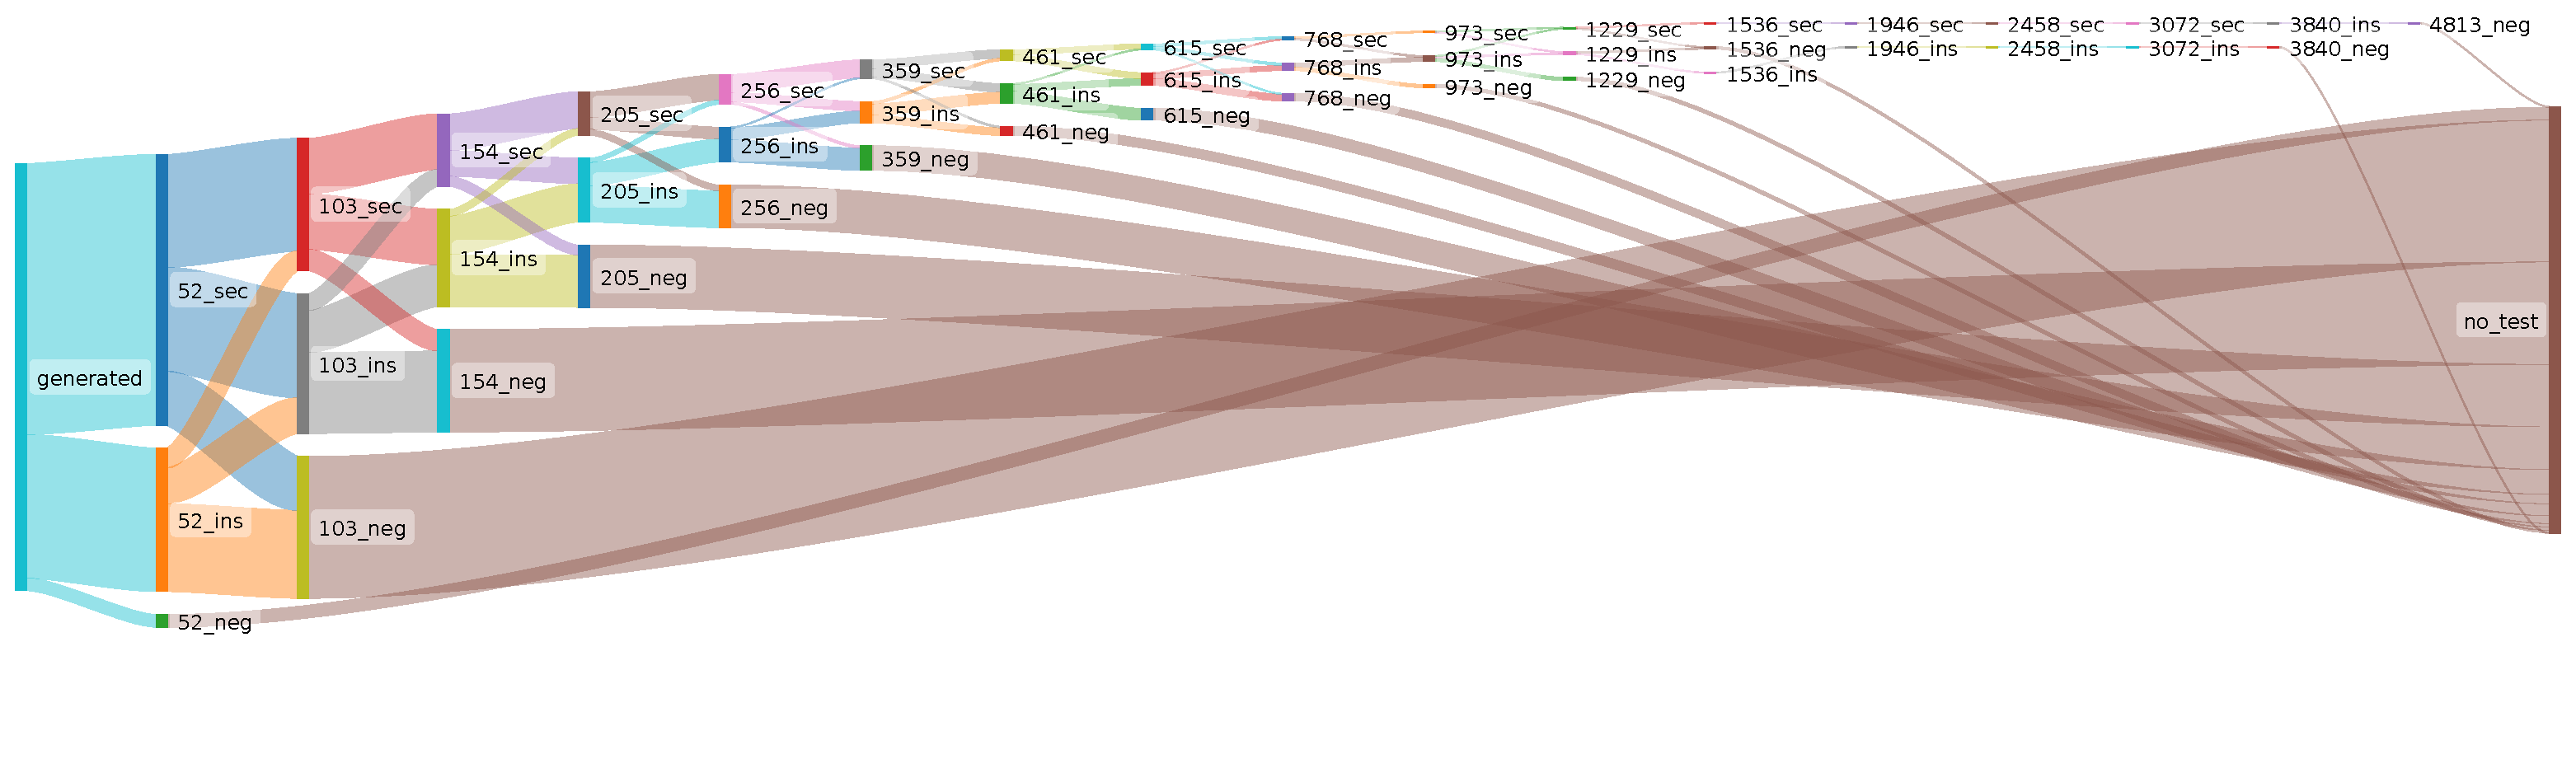
\includegraphics[width=\gsize]{graphs/medium2.old.pdf} \\
    \hline
    \rotatebox{90}{(b). Runtime performance}
  & 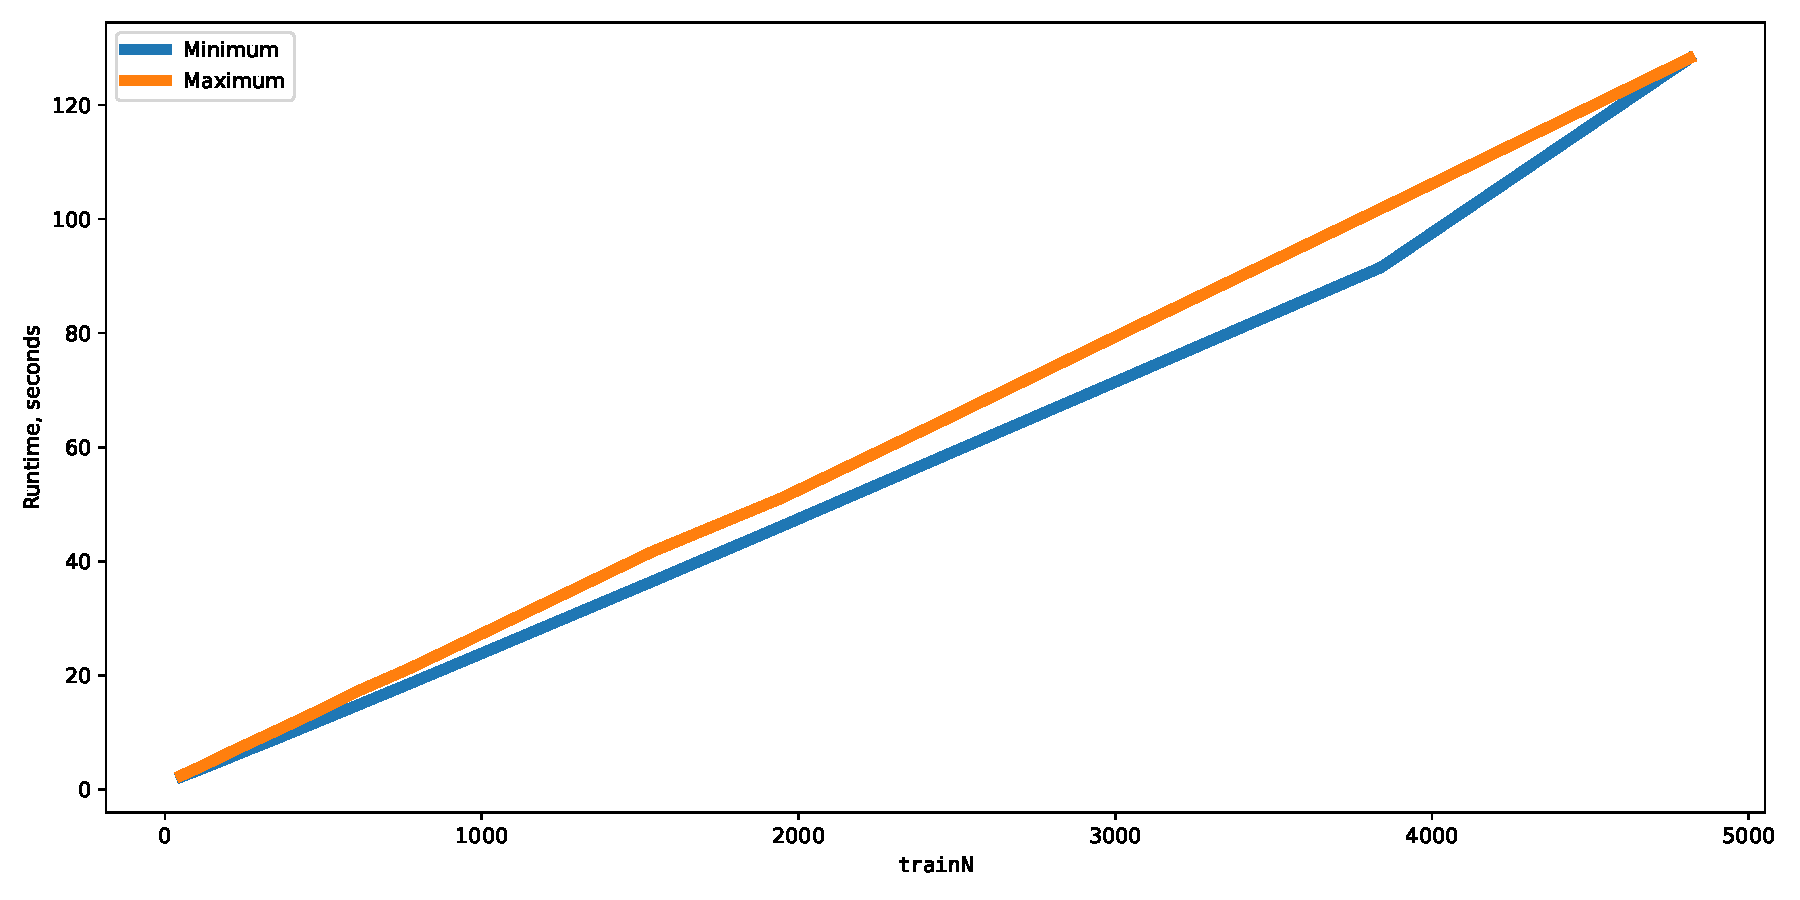
\includegraphics[width=\gsize]{graphs/asymptote_time.pdf} \\
    \hline
    \hline
\end{tabular}
\caption{Experimental results: performance on random protocols.}
\end{figure*}


\subsection{Case-study protocols}
\label{sec:case-study-protocols}

For our evaluation, we implemented three boolean functions, each in two variations of the GMW protocol,
and evaluated \toolname's scalability and ability to find bugs added to these protocols.
The function-circuits and protocols are listed in Table~\ref{tbl:protocols}.
One is a simple addition protocol, three are basic building blocks often used to build more complex protocols, and two are protocols designed to securely evaluate circuits. All six protocols are designed for two parties, with the addition of a third ``dealer'' party to produce correlated randomness in several of the protocols.

\begin{table}
\centering
  \begin{tabular}{|l | l|l|}
    \hline
    \textbf{Protocol} & \textbf{Purpose} & \textbf{Ref.} \\
    \hline
    $n$-bit Addition & Custom & TODO \\
    Oblivious Transfer & Building block & TODO \\
%    OT Extension & Building block & TODO \\
    Beaver Triple Generation & Building block & TODO \\
    GMW & Circuit evaluation & TODO \\
    MPC w/ Beaver Triples & Circuit evaluation & TODO \\
    \hline
  \end{tabular}
  \caption{Secure protocols used in our evaluation.}
  \label{tbl:protocols}
\end{table}

\paragraph{$n$-bit Addition.}
The simplest protocol in our evaluation is a basic summation protocol, which adds up the inputs from the two participating parties. To accomplish this task, the protocol essentially simulates a hardware adder circuit---for each bit in the binary representation of the two input numbers, the protocol performs bitwise operations to compute the sum and carry bit. To ensure security, the input values are \emph{secret shared} using additive secret sharing; to secret share a bit, a party selects a random bit to represent one share, and computes the other share by XORing the random bit with the secret bit. In \langname, $P_1$ can secret share the bit $x$ with $P_2$ as follows:
%
\begin{verbatim}
  s1 = FLIP @P1
  s2 = x + s1
  SEND s1 TO P2
\end{verbatim}
%
$P_1$ can safely send one share to $P_2$, as long as $P_1$ keeps the other share for themselves---neither share alone reveals anything about the secret bit. To add (i.e. XOR) two secret-shared bits, each party can simply add its shares for the two bits to obtain one share of the result. To multiply (i.e. AND) two secret-shared bits, the parties must use oblivious transfer (described next).

Our $n$-bit addition protocol generates a \langname source file for a given bitwidth. In our evaluation, we test several different bitwidths to examine the effect of the size of each party's view on the scalability and bug-finding capability of \toolname.

\begin{figure*}
  \centering
  \newcommand{\gsize}{.45\textwidth}
\begin{tabular}{c| c c}
    \hline\hline
  & \textbf{OT-Based (GMW)} & \textbf{Beaver Triple-Based}\\
    \hline\hline
  \rotatebox{90}{\phantom{hellohello}$n$-bit addition}
  & 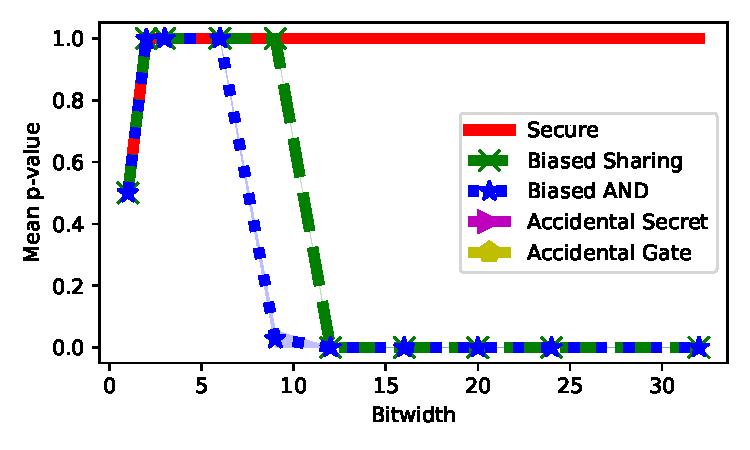
\includegraphics[width=\gsize]{graphs/security_adder_gmw_128_1024.pdf}
                 & 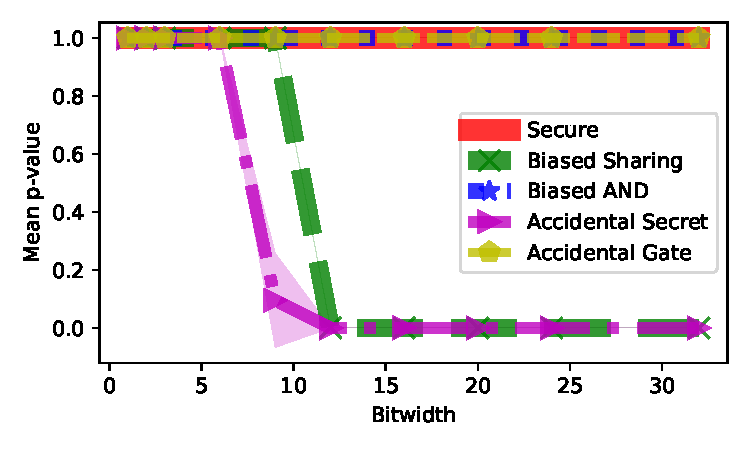
\includegraphics[width=\gsize]{graphs/security_adder_beaver_128_1024.pdf} \\
    \hline
  \rotatebox{90}{\phantom{hel}$n$-bit less-than comparison}
  & 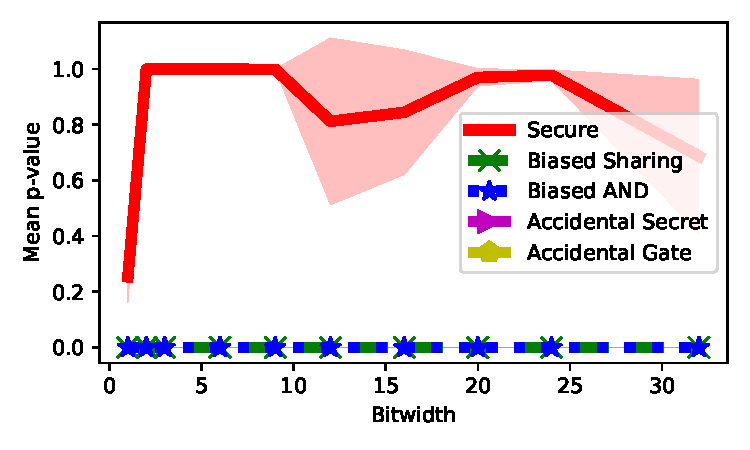
\includegraphics[width=\gsize]{graphs/security_less_than_gmw_128_1024.pdf}
                 & 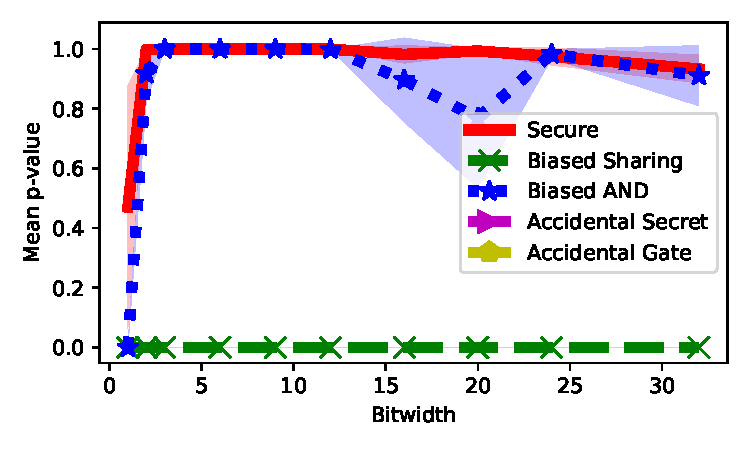
\includegraphics[width=\gsize]{graphs/security_less_than_beaver_128_1024.pdf} \\
    \hline
  \rotatebox{90}{\phantom{h}$n$-bit Beaver triple generation}
  & 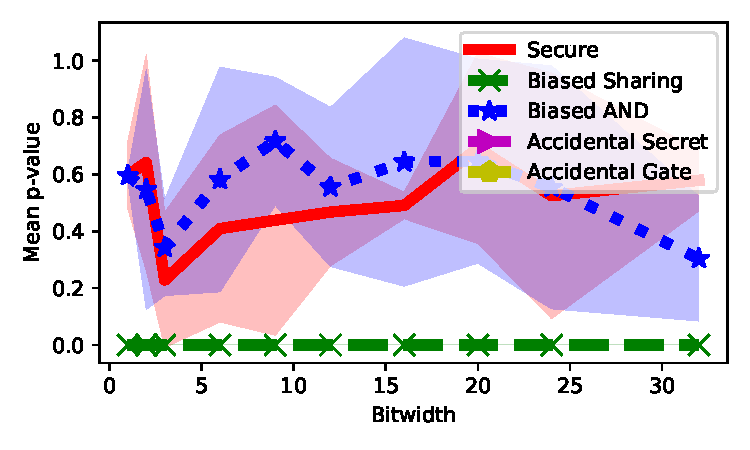
\includegraphics[width=\gsize]{graphs/security_beaver_triple_gen_gmw_128_1024.pdf}
                 & 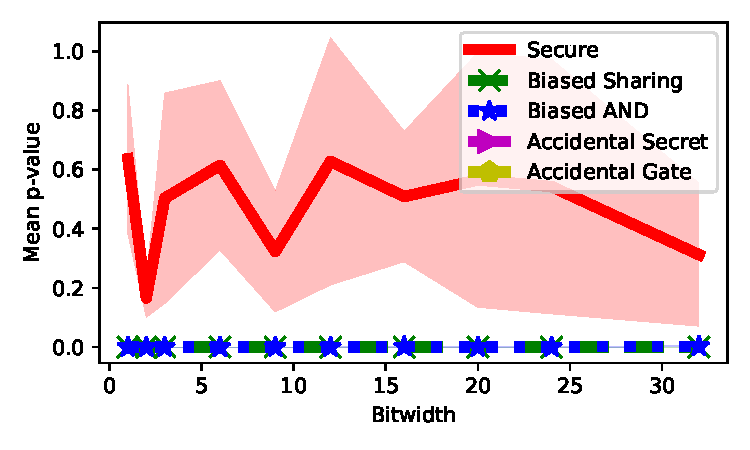
\includegraphics[width=\gsize]{graphs/security_beaver_triple_gen_beaver_128_1024.pdf} \\
    \hline
    \hline
\end{tabular}
\caption{Experimental results: ability to detect security bugs.}
\end{figure*}

\paragraph{Oblivious Transfer.}
Oblivious transfer~\cite{todo} (OT) is a 2-party protocol that allows one party ($R$, the \emph{receiver}) to select one out of several secret inputs provided by the other party ($S$, the \emph{sender}). In 1-out-of-2 OT, $S$ provides 2 secret inputs $x_0$ and $x_1$ and $R$ provides a secret \emph{selection bit} $b$. If $b=0$, $R$ receives $x_0$; if $b=1$, $R$ receives $x_1$. $R$ does not learn anything about the not-selected secret, and $S$ does not learn which secret $R$ selected. This idea can be extended to 1-out-of-$n$ OT by extending the selection bit $b$ to a $\log_2(n)$-bit string.
%
Oblivious transfer is a building block for many other protocols.

% \paragraph{Oblivious Transfer Extension.}
% Protocols like GMW (described later) require the use of OT for each AND gate---for large circuits, this means thousands or millions of OTs. \emph{OT extension}~\cite{todo} is an approach for expanding $k$ ``base'' OTs into $m \gg k$ OTs. OT extension can significantly improve the performance of protocols that use many OTs.

\paragraph{Beaver Triple Generation.}
A \emph{Beaver triple}~\cite{todo} (or \emph{multiplication triple}) is a set of secret shares of numbers $a$, $b$, and $c$ such that $a \cdot b = c$. To use a Beaver triple, $P_1$ must have one share of each of $a$, $b$, and $c$, and $P_2$ must have the other share. Since the values are secret shared, they appear random to each party---but the correlation between the three numbers can be used to perform efficient multiplication between secret-shared numbers (described later). One Beaver triple must be consumed for each multiplication, but they can be generated in a separate offline phase. Beaver triples can be generated by a trusted ``dealer'' party, or by using oblivious transfer. We implement both versions in \langname.

\paragraph{GMW (Goldreich-Micali-Widgerson).}
The GMW protocol is an MPC protocol for evaluating circuits. Each party holds additive secret shares of each wire's value, and evaluates addition gates by adding the shares they hold. The parties evaluate multiplication gates by using 1-out-of-4 oblivious transfer: the first party generates a random bit for its share of the output, and acts as the sender in OT; the second party acts as the receiver in OT and receives its share of the output. We implemented a compiler to generate \langname programs that evaluate  Bristol fashion circuits using GMW, and evaluated it on circuits implementing integer addition and integer inequalities.

\paragraph{MPC with Beaver Triples.}
Another MPC protocol for evaluating circuits also uses additive shares to hold wire values, but uses Beaver triples to evaluate multiplication gates (instead of OT). Given shares of a Beaver triple, the parties perform two multiplication-by-constant and broadcast operations, and derive one share each of the product. Our implementation of this approach employees a third-party ``dealer'' who generates the triples; a pre-processing (offline) phase can also be used to generate the triples. We evaluate \toolname on this protocol using the same circuits as in our GMW experiments.


Our empirical evaluation demonstrates \toolname's ability to detect bugs in secure protocols.
To answer RQ1, we generate \emph{random protocols} of varying sizes, and evaluate \toolname's ability to show they are insecure. The details appear in Section~\ref{sec:experiment-1:-random}. To answer RQ2, we evaluate \toolname on the case study protocols described in Section~\ref{sec:case-study-protocols}. The details appear in Section~\ref{sec:experiment-2:-real}. In both cases, \toolname is able to detect insecurity in the target protocols in under a minute.

\begin{figure*}
  \centering
  \newcommand{\gsize}{.45\textwidth}
\begin{tabular}{c| c c}
    \hline\hline
  & \textbf{OT-Based (GMW)} & \textbf{Beaver Triple-Based}\\
    \hline\hline
  \rotatebox{90}{\phantom{hellohello}$n$-bit addition}
  & 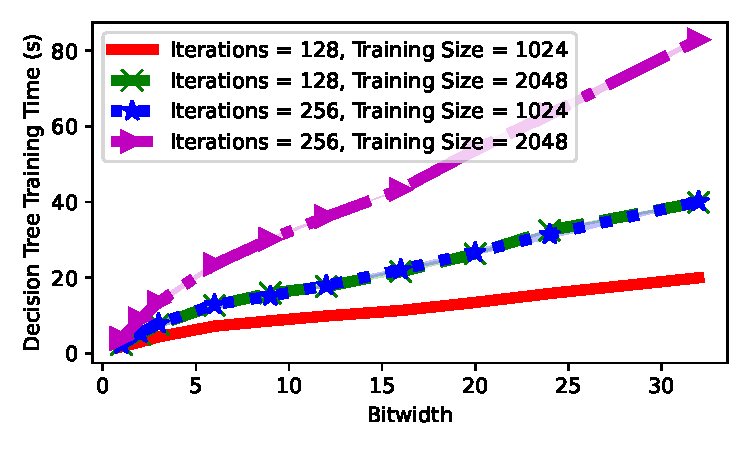
\includegraphics[width=\gsize]{graphs/time_adder_gmw_256_2048.pdf}
                 & 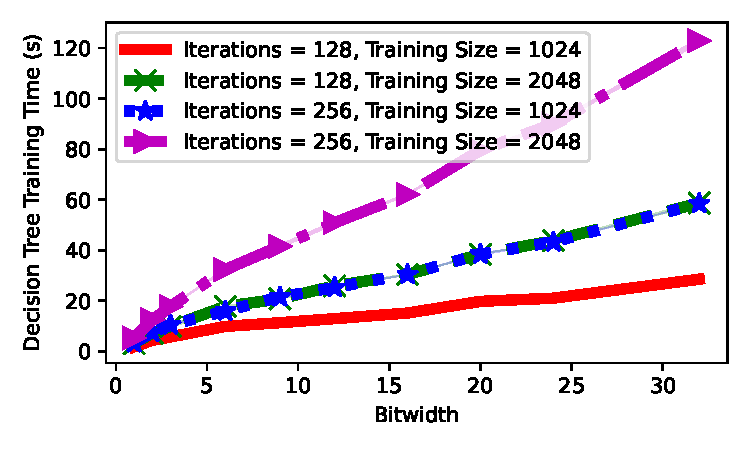
\includegraphics[width=\gsize]{graphs/time_adder_beaver_256_2048.pdf} \\
    \hline
  \rotatebox{90}{\phantom{hel}$n$-bit less-than comparison}
  & 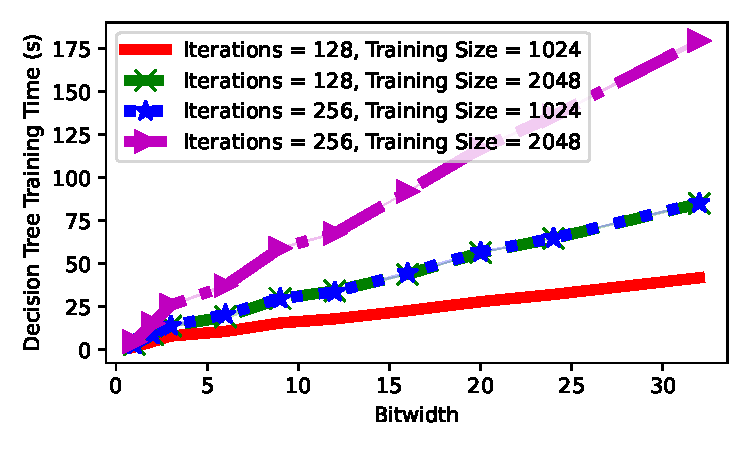
\includegraphics[width=\gsize]{graphs/time_less_than_gmw_256_2048.pdf}
                 & 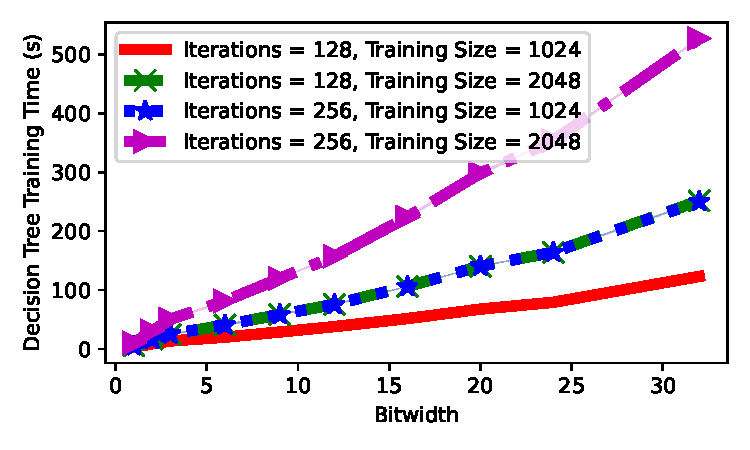
\includegraphics[width=\gsize]{graphs/time_less_than_beaver_256_2048.pdf} \\
    \hline
  \rotatebox{90}{\phantom{h}$n$-bit Beaver triple generation}
  & 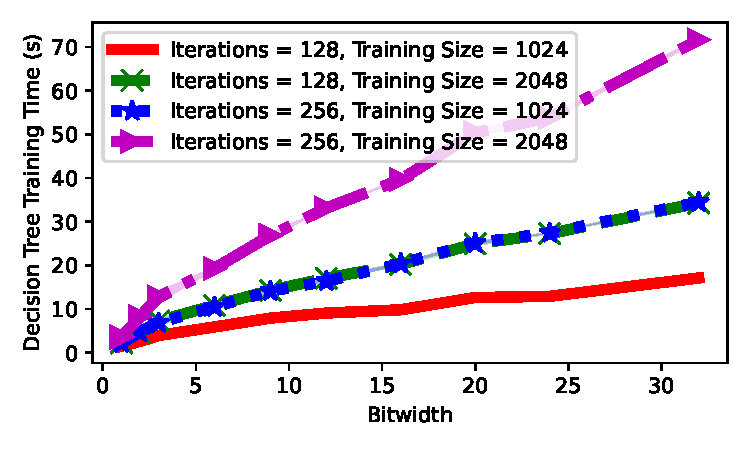
\includegraphics[width=\gsize]{graphs/time_beaver_triple_gen_gmw_256_2048.pdf}
                 & 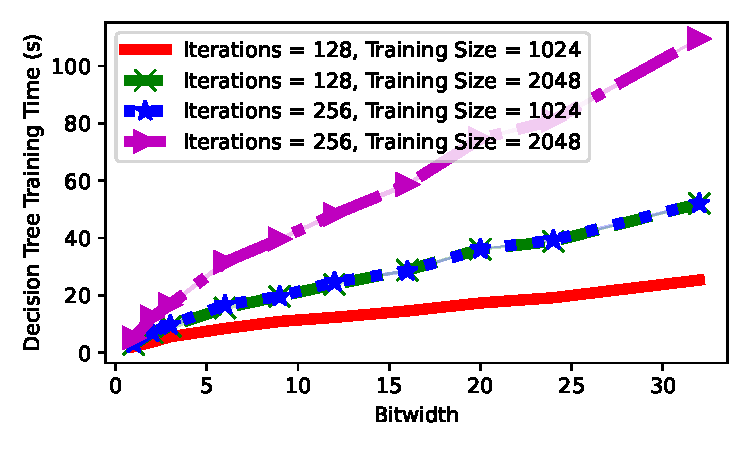
\includegraphics[width=\gsize]{graphs/time_beaver_triple_gen_beaver_256_2048.pdf} \\
    \hline
    \hline
\end{tabular}
\caption{Experimental results: decision tree training time.}
\end{figure*}

\paragraph{Experiment setup.}
In our second experiment, we evaluate \toolname's ability to detect insecurity in the real-world protocols described in Section~\ref{sec:case-study-protocols}. We run \toolname on the unmodified protocol in order to establish that the protocol is secure. Then, we mutate the protocol in several ways to introduce insecurity, and test \toolname's ability to detect it. Specifically, our mutations are:
%
\begin{itemize}
\item \textbf{Accidental secret}: accidentally sends a secret held by the honest party  to the corrupt party.
\item \textbf{Accidental gate}: accidentally sends an honest party's result from the evaluation of a multiplication gate to the corrupt party.
\item \textbf{Biased sharing}: uses biased randomness to construct secret shares of honest party inputs.
\item \textbf{Biased AND}: uses biased randomness as part of the evaluation of multiplication gates.
\end{itemize}
%
The severity of each mutation can be tuned by adjusting the bias in the related randomness. In the case of ``accidental secret'' and ``accidental gate,'' this affects the probability of accidentally revealing a value; in the others, it directly adjust the bias in the randomness.

\paragraph{Results.} \emph{results description goes here}

\subsection{Discussion}




\section{Future Work}


\section{Conclusions}

\bibliographystyle{plain}
\bibliography{refs}

\appendices

\section{Additional Experimental Results}




% These are full figures for the appendix

\begin{figure*}
  \centering
  \newcommand{\gsize}{.45\textwidth}
\begin{tabular}{c| c c}
    \hline\hline
  & \textbf{OT-Based (GMW)} & \textbf{Beaver Triple-Based}\\
    \hline\hline
  \rotatebox{90}{\phantom{helloh}$i = 128, n = 1024$}
  & 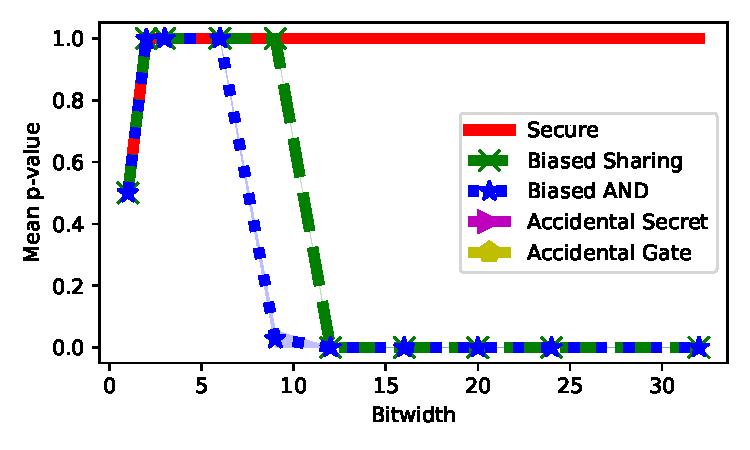
\includegraphics[width=\gsize]{graphs/security_adder_gmw_128_1024.pdf}
                 & 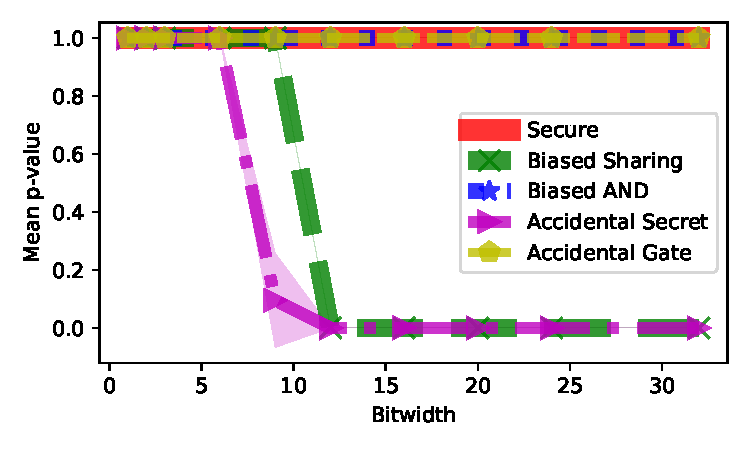
\includegraphics[width=\gsize]{graphs/security_adder_beaver_128_1024.pdf} \\
    \hline
  \rotatebox{90}{\phantom{helloh}$i = 128, n = 2048$}
  & 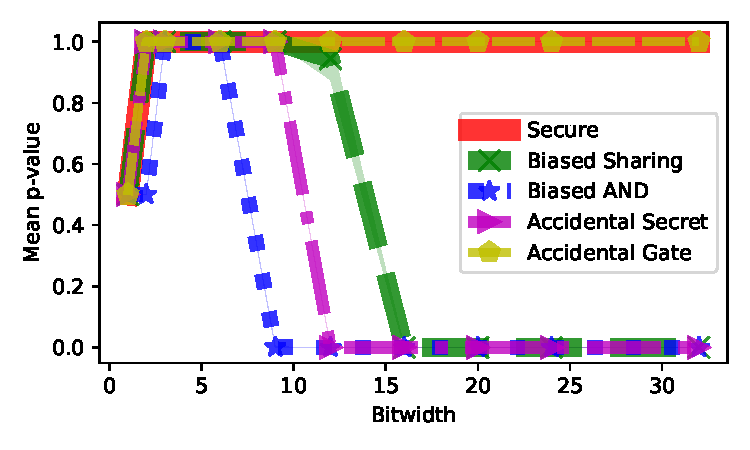
\includegraphics[width=\gsize]{graphs/security_adder_gmw_128_2048.pdf}
                 & 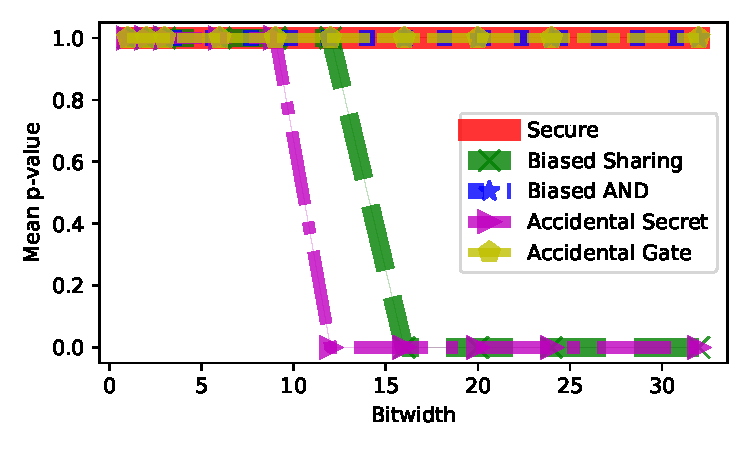
\includegraphics[width=\gsize]{graphs/security_adder_beaver_128_2048.pdf} \\
    \hline
  \rotatebox{90}{\phantom{helloh}$i = 256, n = 1024$}
  & 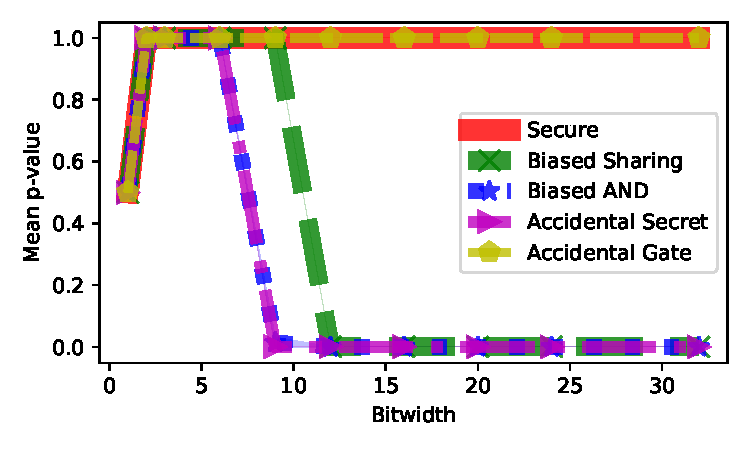
\includegraphics[width=\gsize]{graphs/security_adder_gmw_256_1024.pdf}
                 & 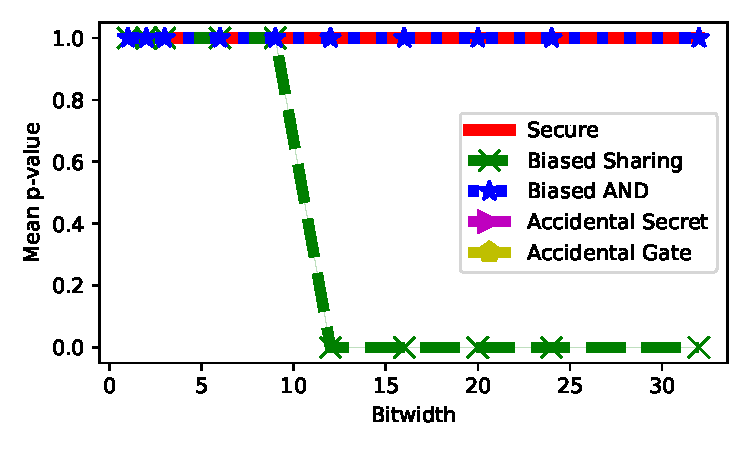
\includegraphics[width=\gsize]{graphs/security_adder_beaver_256_1024.pdf} \\
    \hline
  \rotatebox{90}{\phantom{helloh}$i = 256, n = 2048$}
  & 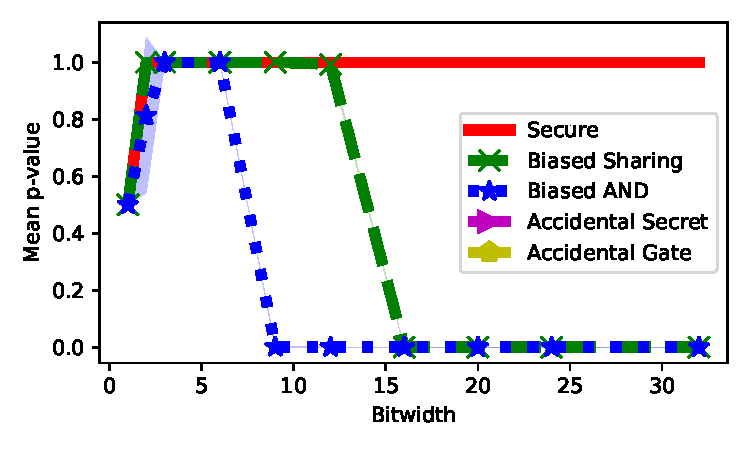
\includegraphics[width=\gsize]{graphs/security_adder_gmw_256_2048.pdf}
                 & 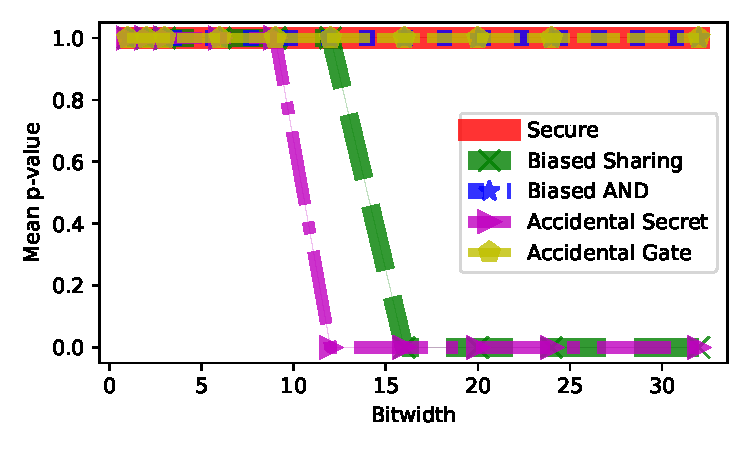
\includegraphics[width=\gsize]{graphs/security_adder_beaver_256_2048.pdf} \\
    \hline
    \hline
\end{tabular}
\caption{Experimental results, $n$-bit addition.}
\end{figure*}

\begin{figure*}
  \centering
  \newcommand{\gsize}{.45\textwidth}
\begin{tabular}{c| c c}
    \hline\hline
  & \textbf{OT-Based (GMW)} & \textbf{Beaver Triple-Based}\\
    \hline\hline
  \rotatebox{90}{\phantom{helloh}$i = 128, n = 1024$}
  & 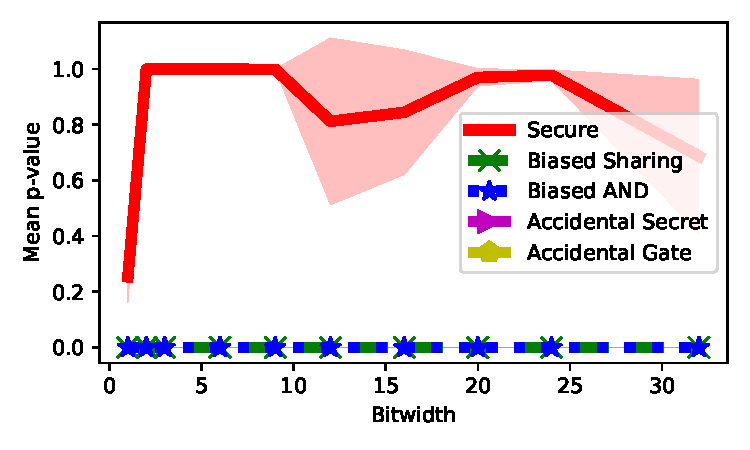
\includegraphics[width=\gsize]{graphs/security_less_than_gmw_128_1024.pdf}
                 & 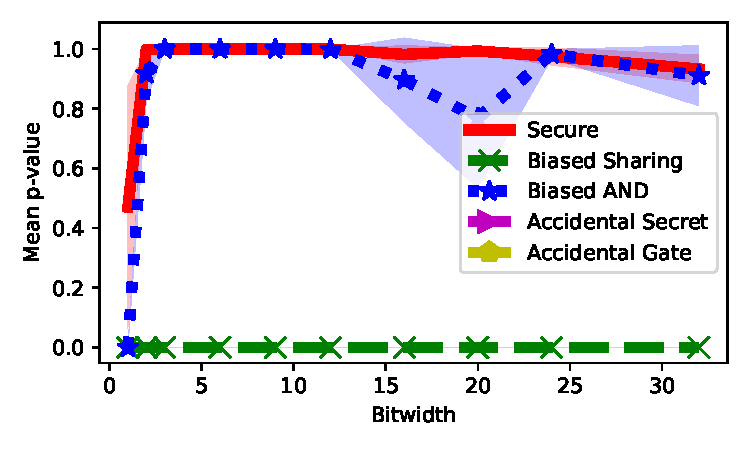
\includegraphics[width=\gsize]{graphs/security_less_than_beaver_128_1024.pdf} \\
    \hline
  \rotatebox{90}{\phantom{helloh}$i = 128, n = 2048$}
  & 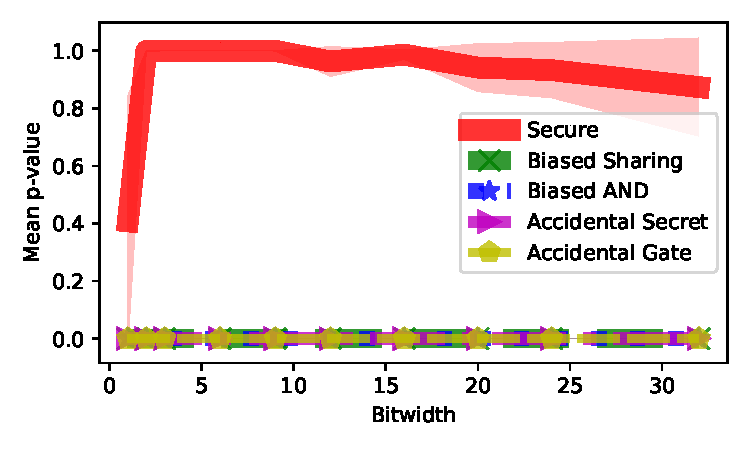
\includegraphics[width=\gsize]{graphs/security_less_than_gmw_128_2048.pdf}
                 & 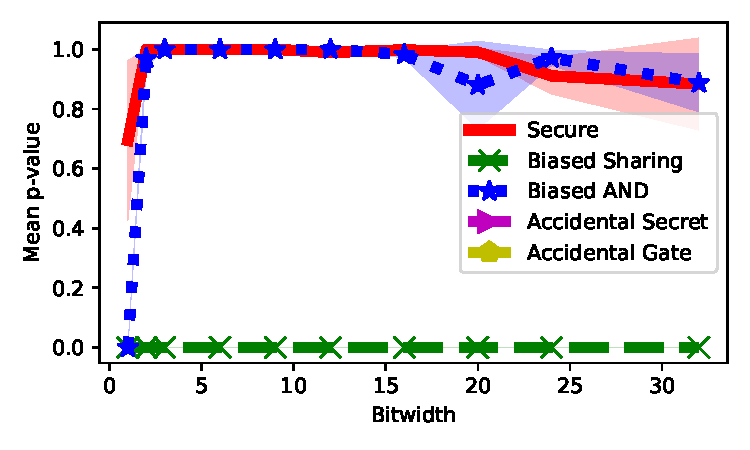
\includegraphics[width=\gsize]{graphs/security_less_than_beaver_128_2048.pdf} \\
    \hline
  \rotatebox{90}{\phantom{helloh}$i = 256, n = 1024$}
  & 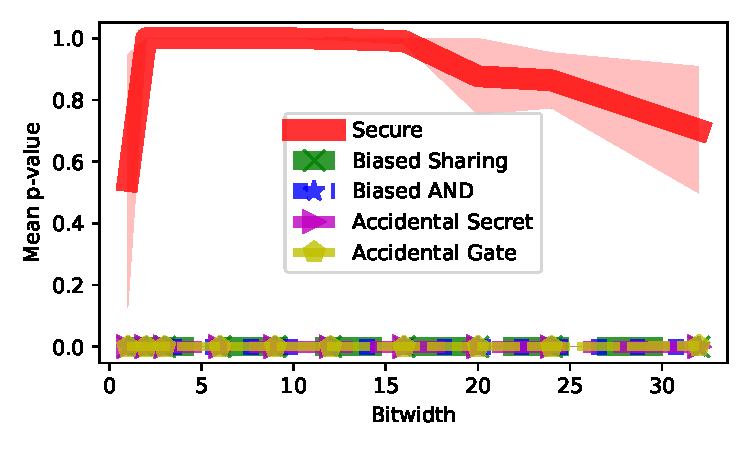
\includegraphics[width=\gsize]{graphs/security_less_than_gmw_256_1024.pdf}
                 & 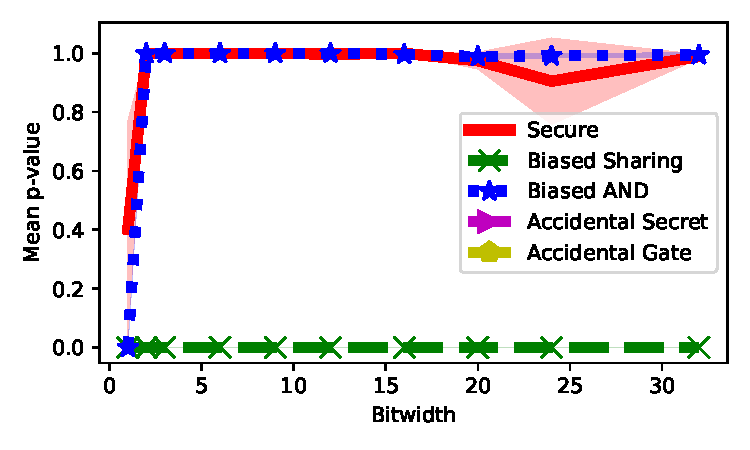
\includegraphics[width=\gsize]{graphs/security_less_than_beaver_256_1024.pdf} \\
    \hline
  \rotatebox{90}{\phantom{helloh}$i = 256, n = 2048$}
  & 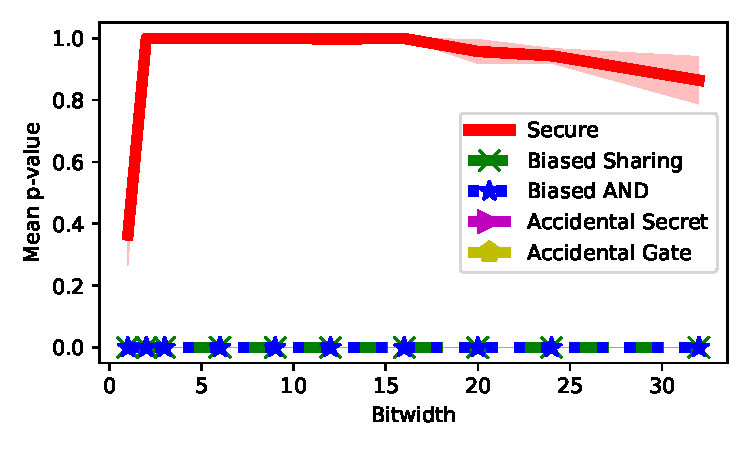
\includegraphics[width=\gsize]{graphs/security_less_than_gmw_256_2048.pdf}
                 & 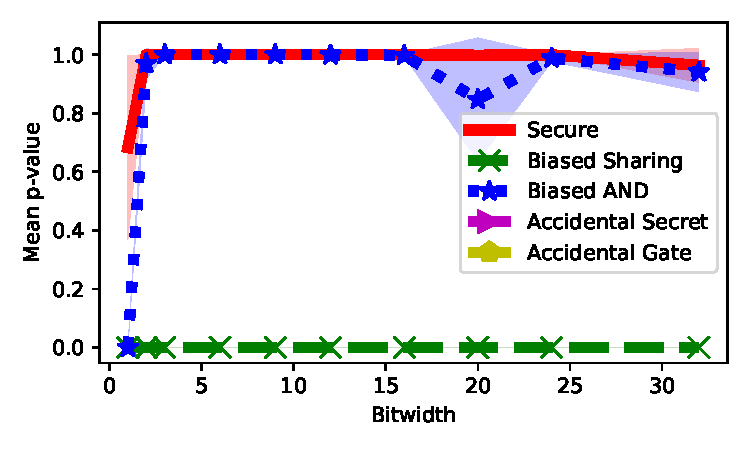
\includegraphics[width=\gsize]{graphs/security_less_than_beaver_256_2048.pdf} \\
    \hline
    \hline
\end{tabular}
\caption{Experimental results, $n$-bit less-than comparison.}
\end{figure*}

\begin{figure*}
  \centering
  \newcommand{\gsize}{.45\textwidth}
\begin{tabular}{c| c c}
    \hline\hline
  & \textbf{OT-Based (GMW)} & \textbf{Beaver Triple-Based}\\
    \hline\hline
  \rotatebox{90}{\phantom{helloh}$i = 128, n = 1024$}
  & 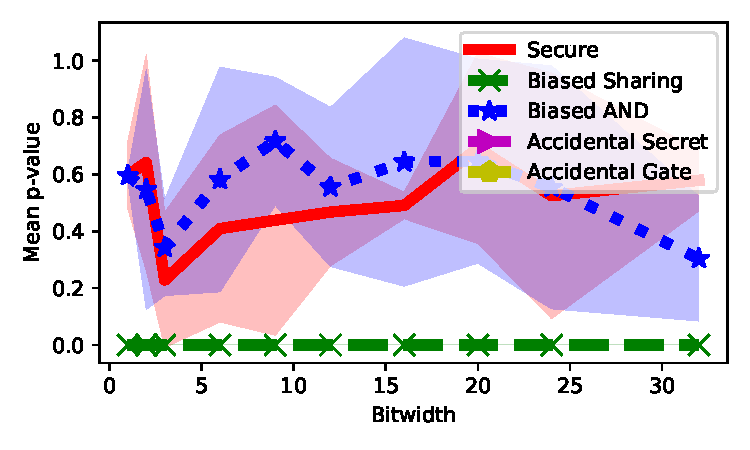
\includegraphics[width=\gsize]{graphs/security_beaver_triple_gen_gmw_128_1024.pdf}
                 & 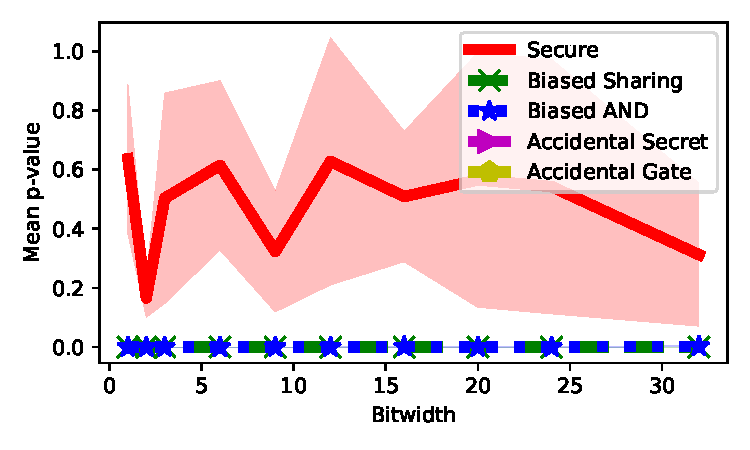
\includegraphics[width=\gsize]{graphs/security_beaver_triple_gen_beaver_128_1024.pdf} \\
    \hline
  \rotatebox{90}{\phantom{helloh}$i = 128, n = 2048$}
  & 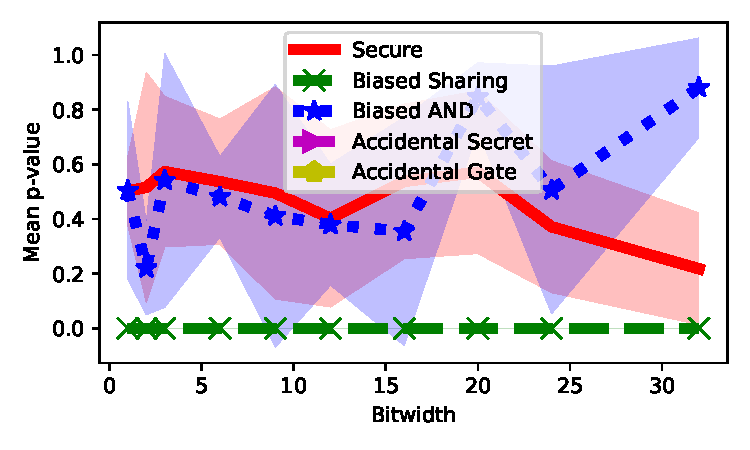
\includegraphics[width=\gsize]{graphs/security_beaver_triple_gen_gmw_128_2048.pdf}
                 & 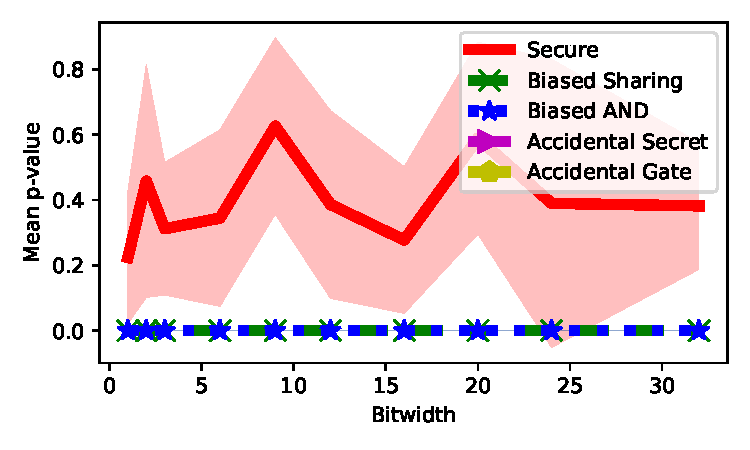
\includegraphics[width=\gsize]{graphs/security_beaver_triple_gen_beaver_128_2048.pdf} \\
    \hline
  \rotatebox{90}{\phantom{helloh}$i = 256, n = 1024$}
  & 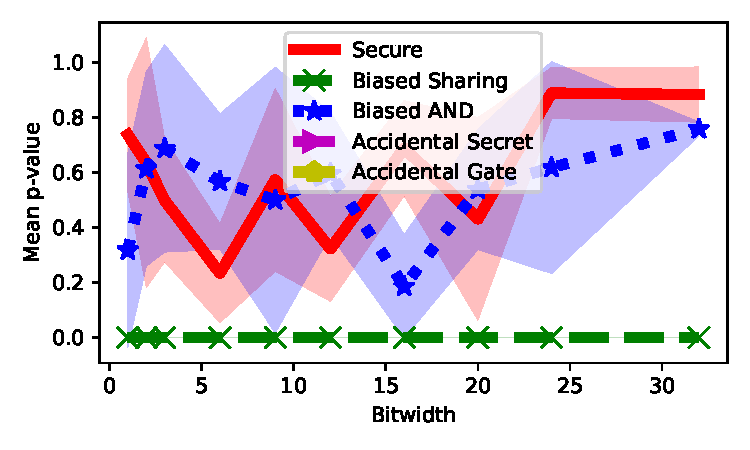
\includegraphics[width=\gsize]{graphs/security_beaver_triple_gen_gmw_256_1024.pdf}
                 & 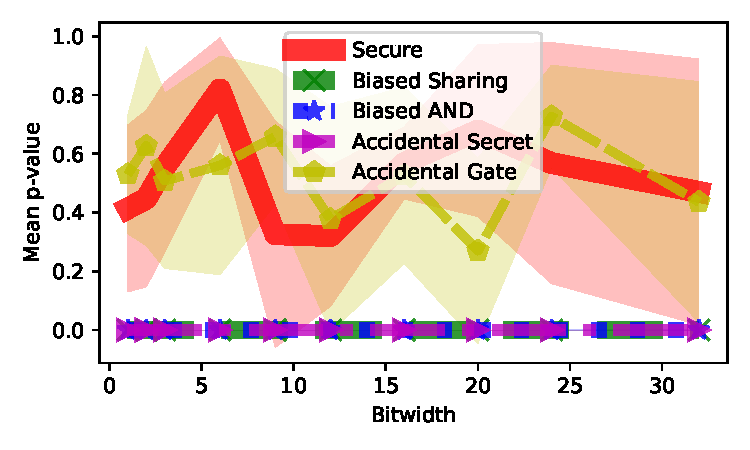
\includegraphics[width=\gsize]{graphs/security_beaver_triple_gen_beaver_256_1024.pdf} \\
    \hline
  \rotatebox{90}{\phantom{helloh}$i = 256, n = 2048$}
  & 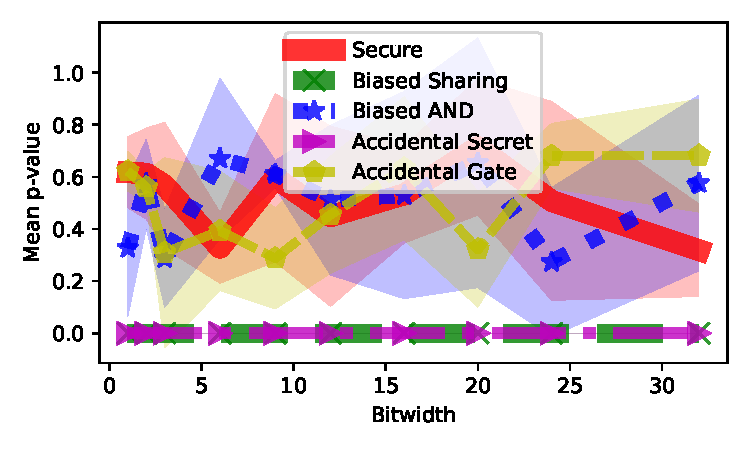
\includegraphics[width=\gsize]{graphs/security_beaver_triple_gen_gmw_256_2048.pdf}
                 & 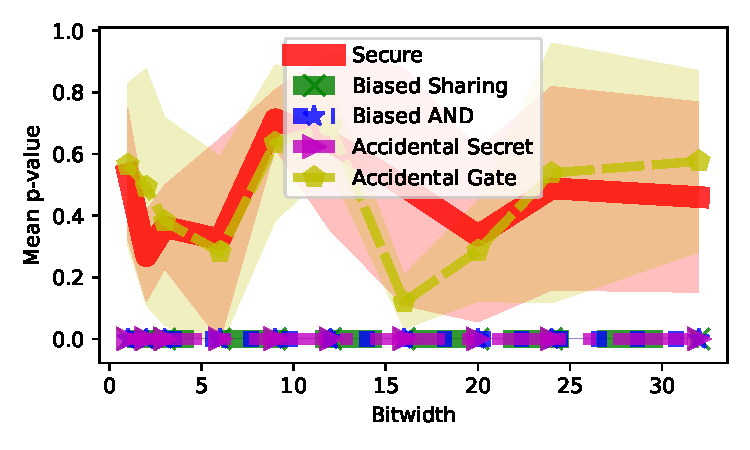
\includegraphics[width=\gsize]{graphs/security_beaver_triple_gen_beaver_256_2048.pdf} \\
    \hline
    \hline
\end{tabular}
\caption{Experimental results, $n$-bit Beaver triple generation.}
\end{figure*}




\end{document}
